
\documentclass{article} % For LaTeX2e
\usepackage{iclr2021_conference,times}

\usepackage{graphicx}
\graphicspath{ {./pics/} }

% Optional math commands from https://github.com/goodfeli/dlbook_notation.
%%%%% NEW MATH DEFINITIONS %%%%%

\usepackage{amsmath,amsfonts,bm}

% Mark sections of captions for referring to divisions of figures
\newcommand{\figleft}{{\em (Left)}}
\newcommand{\figcenter}{{\em (Center)}}
\newcommand{\figright}{{\em (Right)}}
\newcommand{\figtop}{{\em (Top)}}
\newcommand{\figbottom}{{\em (Bottom)}}
\newcommand{\captiona}{{\em (a)}}
\newcommand{\captionb}{{\em (b)}}
\newcommand{\captionc}{{\em (c)}}
\newcommand{\captiond}{{\em (d)}}

% Highlight a newly defined term
\newcommand{\newterm}[1]{{\bf #1}}


% Figure reference, lower-case.
\def\figref#1{figure~\ref{#1}}
% Figure reference, capital. For start of sentence
\def\Figref#1{Figure~\ref{#1}}
\def\twofigref#1#2{figures \ref{#1} and \ref{#2}}
\def\quadfigref#1#2#3#4{figures \ref{#1}, \ref{#2}, \ref{#3} and \ref{#4}}
% Section reference, lower-case.
\def\secref#1{section~\ref{#1}}
% Section reference, capital.
\def\Secref#1{Section~\ref{#1}}
% Reference to two sections.
\def\twosecrefs#1#2{sections \ref{#1} and \ref{#2}}
% Reference to three sections.
\def\secrefs#1#2#3{sections \ref{#1}, \ref{#2} and \ref{#3}}
% Reference to an equation, lower-case.
\def\eqref#1{equation~\ref{#1}}
% Reference to an equation, upper case
\def\Eqref#1{Equation~\ref{#1}}
% A raw reference to an equation---avoid using if possible
\def\plaineqref#1{\ref{#1}}
% Reference to a chapter, lower-case.
\def\chapref#1{chapter~\ref{#1}}
% Reference to an equation, upper case.
\def\Chapref#1{Chapter~\ref{#1}}
% Reference to a range of chapters
\def\rangechapref#1#2{chapters\ref{#1}--\ref{#2}}
% Reference to an algorithm, lower-case.
\def\algref#1{algorithm~\ref{#1}}
% Reference to an algorithm, upper case.
\def\Algref#1{Algorithm~\ref{#1}}
\def\twoalgref#1#2{algorithms \ref{#1} and \ref{#2}}
\def\Twoalgref#1#2{Algorithms \ref{#1} and \ref{#2}}
% Reference to a part, lower case
\def\partref#1{part~\ref{#1}}
% Reference to a part, upper case
\def\Partref#1{Part~\ref{#1}}
\def\twopartref#1#2{parts \ref{#1} and \ref{#2}}

\def\ceil#1{\lceil #1 \rceil}
\def\floor#1{\lfloor #1 \rfloor}
\def\1{\bm{1}}
\newcommand{\train}{\mathcal{D}}
\newcommand{\valid}{\mathcal{D_{\mathrm{valid}}}}
\newcommand{\test}{\mathcal{D_{\mathrm{test}}}}

\def\eps{{\epsilon}}


% Random variables
\def\reta{{\textnormal{$\eta$}}}
\def\ra{{\textnormal{a}}}
\def\rb{{\textnormal{b}}}
\def\rc{{\textnormal{c}}}
\def\rd{{\textnormal{d}}}
\def\re{{\textnormal{e}}}
\def\rf{{\textnormal{f}}}
\def\rg{{\textnormal{g}}}
\def\rh{{\textnormal{h}}}
\def\ri{{\textnormal{i}}}
\def\rj{{\textnormal{j}}}
\def\rk{{\textnormal{k}}}
\def\rl{{\textnormal{l}}}
% rm is already a command, just don't name any random variables m
\def\rn{{\textnormal{n}}}
\def\ro{{\textnormal{o}}}
\def\rp{{\textnormal{p}}}
\def\rq{{\textnormal{q}}}
\def\rr{{\textnormal{r}}}
\def\rs{{\textnormal{s}}}
\def\rt{{\textnormal{t}}}
\def\ru{{\textnormal{u}}}
\def\rv{{\textnormal{v}}}
\def\rw{{\textnormal{w}}}
\def\rx{{\textnormal{x}}}
\def\ry{{\textnormal{y}}}
\def\rz{{\textnormal{z}}}

% Random vectors
\def\rvepsilon{{\mathbf{\epsilon}}}
\def\rvtheta{{\mathbf{\theta}}}
\def\rva{{\mathbf{a}}}
\def\rvb{{\mathbf{b}}}
\def\rvc{{\mathbf{c}}}
\def\rvd{{\mathbf{d}}}
\def\rve{{\mathbf{e}}}
\def\rvf{{\mathbf{f}}}
\def\rvg{{\mathbf{g}}}
\def\rvh{{\mathbf{h}}}
\def\rvu{{\mathbf{i}}}
\def\rvj{{\mathbf{j}}}
\def\rvk{{\mathbf{k}}}
\def\rvl{{\mathbf{l}}}
\def\rvm{{\mathbf{m}}}
\def\rvn{{\mathbf{n}}}
\def\rvo{{\mathbf{o}}}
\def\rvp{{\mathbf{p}}}
\def\rvq{{\mathbf{q}}}
\def\rvr{{\mathbf{r}}}
\def\rvs{{\mathbf{s}}}
\def\rvt{{\mathbf{t}}}
\def\rvu{{\mathbf{u}}}
\def\rvv{{\mathbf{v}}}
\def\rvw{{\mathbf{w}}}
\def\rvx{{\mathbf{x}}}
\def\rvy{{\mathbf{y}}}
\def\rvz{{\mathbf{z}}}

% Elements of random vectors
\def\erva{{\textnormal{a}}}
\def\ervb{{\textnormal{b}}}
\def\ervc{{\textnormal{c}}}
\def\ervd{{\textnormal{d}}}
\def\erve{{\textnormal{e}}}
\def\ervf{{\textnormal{f}}}
\def\ervg{{\textnormal{g}}}
\def\ervh{{\textnormal{h}}}
\def\ervi{{\textnormal{i}}}
\def\ervj{{\textnormal{j}}}
\def\ervk{{\textnormal{k}}}
\def\ervl{{\textnormal{l}}}
\def\ervm{{\textnormal{m}}}
\def\ervn{{\textnormal{n}}}
\def\ervo{{\textnormal{o}}}
\def\ervp{{\textnormal{p}}}
\def\ervq{{\textnormal{q}}}
\def\ervr{{\textnormal{r}}}
\def\ervs{{\textnormal{s}}}
\def\ervt{{\textnormal{t}}}
\def\ervu{{\textnormal{u}}}
\def\ervv{{\textnormal{v}}}
\def\ervw{{\textnormal{w}}}
\def\ervx{{\textnormal{x}}}
\def\ervy{{\textnormal{y}}}
\def\ervz{{\textnormal{z}}}

% Random matrices
\def\rmA{{\mathbf{A}}}
\def\rmB{{\mathbf{B}}}
\def\rmC{{\mathbf{C}}}
\def\rmD{{\mathbf{D}}}
\def\rmE{{\mathbf{E}}}
\def\rmF{{\mathbf{F}}}
\def\rmG{{\mathbf{G}}}
\def\rmH{{\mathbf{H}}}
\def\rmI{{\mathbf{I}}}
\def\rmJ{{\mathbf{J}}}
\def\rmK{{\mathbf{K}}}
\def\rmL{{\mathbf{L}}}
\def\rmM{{\mathbf{M}}}
\def\rmN{{\mathbf{N}}}
\def\rmO{{\mathbf{O}}}
\def\rmP{{\mathbf{P}}}
\def\rmQ{{\mathbf{Q}}}
\def\rmR{{\mathbf{R}}}
\def\rmS{{\mathbf{S}}}
\def\rmT{{\mathbf{T}}}
\def\rmU{{\mathbf{U}}}
\def\rmV{{\mathbf{V}}}
\def\rmW{{\mathbf{W}}}
\def\rmX{{\mathbf{X}}}
\def\rmY{{\mathbf{Y}}}
\def\rmZ{{\mathbf{Z}}}

% Elements of random matrices
\def\ermA{{\textnormal{A}}}
\def\ermB{{\textnormal{B}}}
\def\ermC{{\textnormal{C}}}
\def\ermD{{\textnormal{D}}}
\def\ermE{{\textnormal{E}}}
\def\ermF{{\textnormal{F}}}
\def\ermG{{\textnormal{G}}}
\def\ermH{{\textnormal{H}}}
\def\ermI{{\textnormal{I}}}
\def\ermJ{{\textnormal{J}}}
\def\ermK{{\textnormal{K}}}
\def\ermL{{\textnormal{L}}}
\def\ermM{{\textnormal{M}}}
\def\ermN{{\textnormal{N}}}
\def\ermO{{\textnormal{O}}}
\def\ermP{{\textnormal{P}}}
\def\ermQ{{\textnormal{Q}}}
\def\ermR{{\textnormal{R}}}
\def\ermS{{\textnormal{S}}}
\def\ermT{{\textnormal{T}}}
\def\ermU{{\textnormal{U}}}
\def\ermV{{\textnormal{V}}}
\def\ermW{{\textnormal{W}}}
\def\ermX{{\textnormal{X}}}
\def\ermY{{\textnormal{Y}}}
\def\ermZ{{\textnormal{Z}}}

% Vectors
\def\vzero{{\bm{0}}}
\def\vone{{\bm{1}}}
\def\vmu{{\bm{\mu}}}
\def\vtheta{{\bm{\theta}}}
\def\va{{\bm{a}}}
\def\vb{{\bm{b}}}
\def\vc{{\bm{c}}}
\def\vd{{\bm{d}}}
\def\ve{{\bm{e}}}
\def\vf{{\bm{f}}}
\def\vg{{\bm{g}}}
\def\vh{{\bm{h}}}
\def\vi{{\bm{i}}}
\def\vj{{\bm{j}}}
\def\vk{{\bm{k}}}
\def\vl{{\bm{l}}}
\def\vm{{\bm{m}}}
\def\vn{{\bm{n}}}
\def\vo{{\bm{o}}}
\def\vp{{\bm{p}}}
\def\vq{{\bm{q}}}
\def\vr{{\bm{r}}}
\def\vs{{\bm{s}}}
\def\vt{{\bm{t}}}
\def\vu{{\bm{u}}}
\def\vv{{\bm{v}}}
\def\vw{{\bm{w}}}
\def\vx{{\bm{x}}}
\def\vy{{\bm{y}}}
\def\vz{{\bm{z}}}

% Elements of vectors
\def\evalpha{{\alpha}}
\def\evbeta{{\beta}}
\def\evepsilon{{\epsilon}}
\def\evlambda{{\lambda}}
\def\evomega{{\omega}}
\def\evmu{{\mu}}
\def\evpsi{{\psi}}
\def\evsigma{{\sigma}}
\def\evtheta{{\theta}}
\def\eva{{a}}
\def\evb{{b}}
\def\evc{{c}}
\def\evd{{d}}
\def\eve{{e}}
\def\evf{{f}}
\def\evg{{g}}
\def\evh{{h}}
\def\evi{{i}}
\def\evj{{j}}
\def\evk{{k}}
\def\evl{{l}}
\def\evm{{m}}
\def\evn{{n}}
\def\evo{{o}}
\def\evp{{p}}
\def\evq{{q}}
\def\evr{{r}}
\def\evs{{s}}
\def\evt{{t}}
\def\evu{{u}}
\def\evv{{v}}
\def\evw{{w}}
\def\evx{{x}}
\def\evy{{y}}
\def\evz{{z}}

% Matrix
\def\mA{{\bm{A}}}
\def\mB{{\bm{B}}}
\def\mC{{\bm{C}}}
\def\mD{{\bm{D}}}
\def\mE{{\bm{E}}}
\def\mF{{\bm{F}}}
\def\mG{{\bm{G}}}
\def\mH{{\bm{H}}}
\def\mI{{\bm{I}}}
\def\mJ{{\bm{J}}}
\def\mK{{\bm{K}}}
\def\mL{{\bm{L}}}
\def\mM{{\bm{M}}}
\def\mN{{\bm{N}}}
\def\mO{{\bm{O}}}
\def\mP{{\bm{P}}}
\def\mQ{{\bm{Q}}}
\def\mR{{\bm{R}}}
\def\mS{{\bm{S}}}
\def\mT{{\bm{T}}}
\def\mU{{\bm{U}}}
\def\mV{{\bm{V}}}
\def\mW{{\bm{W}}}
\def\mX{{\bm{X}}}
\def\mY{{\bm{Y}}}
\def\mZ{{\bm{Z}}}
\def\mBeta{{\bm{\beta}}}
\def\mPhi{{\bm{\Phi}}}
\def\mLambda{{\bm{\Lambda}}}
\def\mSigma{{\bm{\Sigma}}}

% Tensor
\DeclareMathAlphabet{\mathsfit}{\encodingdefault}{\sfdefault}{m}{sl}
\SetMathAlphabet{\mathsfit}{bold}{\encodingdefault}{\sfdefault}{bx}{n}
\newcommand{\tens}[1]{\bm{\mathsfit{#1}}}
\def\tA{{\tens{A}}}
\def\tB{{\tens{B}}}
\def\tC{{\tens{C}}}
\def\tD{{\tens{D}}}
\def\tE{{\tens{E}}}
\def\tF{{\tens{F}}}
\def\tG{{\tens{G}}}
\def\tH{{\tens{H}}}
\def\tI{{\tens{I}}}
\def\tJ{{\tens{J}}}
\def\tK{{\tens{K}}}
\def\tL{{\tens{L}}}
\def\tM{{\tens{M}}}
\def\tN{{\tens{N}}}
\def\tO{{\tens{O}}}
\def\tP{{\tens{P}}}
\def\tQ{{\tens{Q}}}
\def\tR{{\tens{R}}}
\def\tS{{\tens{S}}}
\def\tT{{\tens{T}}}
\def\tU{{\tens{U}}}
\def\tV{{\tens{V}}}
\def\tW{{\tens{W}}}
\def\tX{{\tens{X}}}
\def\tY{{\tens{Y}}}
\def\tZ{{\tens{Z}}}


% Graph
\def\gA{{\mathcal{A}}}
\def\gB{{\mathcal{B}}}
\def\gC{{\mathcal{C}}}
\def\gD{{\mathcal{D}}}
\def\gE{{\mathcal{E}}}
\def\gF{{\mathcal{F}}}
\def\gG{{\mathcal{G}}}
\def\gH{{\mathcal{H}}}
\def\gI{{\mathcal{I}}}
\def\gJ{{\mathcal{J}}}
\def\gK{{\mathcal{K}}}
\def\gL{{\mathcal{L}}}
\def\gM{{\mathcal{M}}}
\def\gN{{\mathcal{N}}}
\def\gO{{\mathcal{O}}}
\def\gP{{\mathcal{P}}}
\def\gQ{{\mathcal{Q}}}
\def\gR{{\mathcal{R}}}
\def\gS{{\mathcal{S}}}
\def\gT{{\mathcal{T}}}
\def\gU{{\mathcal{U}}}
\def\gV{{\mathcal{V}}}
\def\gW{{\mathcal{W}}}
\def\gX{{\mathcal{X}}}
\def\gY{{\mathcal{Y}}}
\def\gZ{{\mathcal{Z}}}

% Sets
\def\sA{{\mathbb{A}}}
\def\sB{{\mathbb{B}}}
\def\sC{{\mathbb{C}}}
\def\sD{{\mathbb{D}}}
% Don't use a set called E, because this would be the same as our symbol
% for expectation.
\def\sF{{\mathbb{F}}}
\def\sG{{\mathbb{G}}}
\def\sH{{\mathbb{H}}}
\def\sI{{\mathbb{I}}}
\def\sJ{{\mathbb{J}}}
\def\sK{{\mathbb{K}}}
\def\sL{{\mathbb{L}}}
\def\sM{{\mathbb{M}}}
\def\sN{{\mathbb{N}}}
\def\sO{{\mathbb{O}}}
\def\sP{{\mathbb{P}}}
\def\sQ{{\mathbb{Q}}}
\def\sR{{\mathbb{R}}}
\def\sS{{\mathbb{S}}}
\def\sT{{\mathbb{T}}}
\def\sU{{\mathbb{U}}}
\def\sV{{\mathbb{V}}}
\def\sW{{\mathbb{W}}}
\def\sX{{\mathbb{X}}}
\def\sY{{\mathbb{Y}}}
\def\sZ{{\mathbb{Z}}}

% Entries of a matrix
\def\emLambda{{\Lambda}}
\def\emA{{A}}
\def\emB{{B}}
\def\emC{{C}}
\def\emD{{D}}
\def\emE{{E}}
\def\emF{{F}}
\def\emG{{G}}
\def\emH{{H}}
\def\emI{{I}}
\def\emJ{{J}}
\def\emK{{K}}
\def\emL{{L}}
\def\emM{{M}}
\def\emN{{N}}
\def\emO{{O}}
\def\emP{{P}}
\def\emQ{{Q}}
\def\emR{{R}}
\def\emS{{S}}
\def\emT{{T}}
\def\emU{{U}}
\def\emV{{V}}
\def\emW{{W}}
\def\emX{{X}}
\def\emY{{Y}}
\def\emZ{{Z}}
\def\emSigma{{\Sigma}}

% entries of a tensor
% Same font as tensor, without \bm wrapper
\newcommand{\etens}[1]{\mathsfit{#1}}
\def\etLambda{{\etens{\Lambda}}}
\def\etA{{\etens{A}}}
\def\etB{{\etens{B}}}
\def\etC{{\etens{C}}}
\def\etD{{\etens{D}}}
\def\etE{{\etens{E}}}
\def\etF{{\etens{F}}}
\def\etG{{\etens{G}}}
\def\etH{{\etens{H}}}
\def\etI{{\etens{I}}}
\def\etJ{{\etens{J}}}
\def\etK{{\etens{K}}}
\def\etL{{\etens{L}}}
\def\etM{{\etens{M}}}
\def\etN{{\etens{N}}}
\def\etO{{\etens{O}}}
\def\etP{{\etens{P}}}
\def\etQ{{\etens{Q}}}
\def\etR{{\etens{R}}}
\def\etS{{\etens{S}}}
\def\etT{{\etens{T}}}
\def\etU{{\etens{U}}}
\def\etV{{\etens{V}}}
\def\etW{{\etens{W}}}
\def\etX{{\etens{X}}}
\def\etY{{\etens{Y}}}
\def\etZ{{\etens{Z}}}

% The true underlying data generating distribution
\newcommand{\pdata}{p_{\rm{data}}}
% The empirical distribution defined by the training set
\newcommand{\ptrain}{\hat{p}_{\rm{data}}}
\newcommand{\Ptrain}{\hat{P}_{\rm{data}}}
% The model distribution
\newcommand{\pmodel}{p_{\rm{model}}}
\newcommand{\Pmodel}{P_{\rm{model}}}
\newcommand{\ptildemodel}{\tilde{p}_{\rm{model}}}
% Stochastic autoencoder distributions
\newcommand{\pencode}{p_{\rm{encoder}}}
\newcommand{\pdecode}{p_{\rm{decoder}}}
\newcommand{\precons}{p_{\rm{reconstruct}}}

\newcommand{\laplace}{\mathrm{Laplace}} % Laplace distribution

\newcommand{\E}{\mathbb{E}}
\newcommand{\Ls}{\mathcal{L}}
\newcommand{\R}{\mathbb{R}}
\newcommand{\emp}{\tilde{p}}
\newcommand{\lr}{\alpha}
\newcommand{\reg}{\lambda}
\newcommand{\rect}{\mathrm{rectifier}}
\newcommand{\softmax}{\mathrm{softmax}}
\newcommand{\sigmoid}{\sigma}
\newcommand{\softplus}{\zeta}
\newcommand{\KL}{D_{\mathrm{KL}}}
\newcommand{\Var}{\mathrm{Var}}
\newcommand{\standarderror}{\mathrm{SE}}
\newcommand{\Cov}{\mathrm{Cov}}
% Wolfram Mathworld says $L^2$ is for function spaces and $\ell^2$ is for vectors
% But then they seem to use $L^2$ for vectors throughout the site, and so does
% wikipedia.
\newcommand{\normlzero}{L^0}
\newcommand{\normlone}{L^1}
\newcommand{\normltwo}{L^2}
\newcommand{\normlp}{L^p}
\newcommand{\normmax}{L^\infty}

\newcommand{\parents}{Pa} % See usage in notation.tex. Chosen to match Daphne's book.

\DeclareMathOperator*{\argmax}{arg\,max}
\DeclareMathOperator*{\argmin}{arg\,min}

\DeclareMathOperator{\sign}{sign}
\DeclareMathOperator{\Tr}{Tr}
\let\ab\allowbreak

% differential
\renewcommand{\rvx}{\mathtt{x}}
\renewcommand{\rvc}{\mathtt{c}}
\renewcommand{\rvz}{\mathtt{z}}
\newcommand{\dd}{\, \textnormal{d}}
\newcommand{\Lsh}{\widehat{\Ls}}
\newcommand{\pc}{p_c}
\newcommand{\qc}{q_c}
\newcommand{\mux}{\mu_x}
\newcommand{\muc}{\mu_c}
\newcommand{\Hc}{\sH_{\muc}}
\newcommand{\cHc}{\sH_{\muc|\qc}}
\newcommand{\gEt}{\gE_\theta}
\newcommand{\gQE}{\gQ_\mE}
\newcommand{\gDp}{\gD_\phi}
\newcommand{\gTEt}{\gT_{\mE, \theta}}
\newcommand{\vzb}{\bar{\vz}}
\newcommand{\vzh}{\hat{\vz}}
\newcommand{\vzt}{\tilde{\vz}}
\newcommand{\vxh}{\hat{\vx}}
\newcommand{\gPp}{\gP_{\psi}}
\newcommand{\vct}{\tilde{\vc}}

\usepackage{hyperref}
\usepackage{url}


\title{Learned transform compression with optimized entropy encoding.}

% Authors must not appear in the submitted version. They should be hidden
% as long as the \iclrfinalcopy macro remains commented out below.
% Non-anonymous submissions will be rejected without review.

\author{Magda Gregorová \& Marc Desaules \& Alexandros Kalousis \\
Geneva School of Business Administration, HES-SO \\
Carouge, Swizerland \\
\texttt{\{name.surname\}@hesge.ch} \\
}

% The \author macro works with any number of authors. There are two commands
% used to separate the names and addresses of multiple authors: \And and \AND.
%
% Using \And between authors leaves it to \LaTeX{} to determine where to break
% the lines. Using \AND forces a linebreak at that point. So, if \LaTeX{}
% puts 3 of 4 authors names on the first line, and the last on the second
% line, try using \AND instead of \And before the third author name.

\newcommand{\fix}{\marginpar{FIX}}
\newcommand{\new}{\marginpar{NEW}}

% \iclrfinalcopy % Uncomment for camera-ready version, but NOT for submission.
\begin{document}


\maketitle

\begin{abstract}
We consider the problem of learned transform compression where we learn both, the transform as well as the probability distribution over the discrete codes.
\end{abstract}

\section{Introduction}\label{sec:Intro}

We consider the problem of compressing data $\vx \in \sX$ sampled i.i.d. according to some unknown probability measure (distribution) $\vx \sim \mux$\footnote{For the sake of generality, we do not take any assumptions about the probability space being discrete or continuous.}.
We take the standard transform coding \citep{sayoodIntroductionDataCompression2012} approach to compression where we first transform the data by a learned non-linear function, an encoder $\gEt : \sX \to \sZ$, into some latent representation $\vz \in \sZ$.
We then quantize the transformed data $\vz = \gEt(\vx)$ using a quantization function $\gQE : \sZ \to \sC$ parametrized by a learned embedding $\mE$ (codebook/ dictionary) so that the discrete codes composed of indexes of the embedding vectors $\vc = \gQE(\vz)$ can be compressed by a lossless entropy encoding and transmitted.
The received and losslessly decoded integer codes are then used to index the embedding vectors and dequantize back to the latent space $\overline{\gQE} : \sC \to \widehat{\sZ} \subset \sZ$ introducing a distortion due to mapping the codes only to the discrete subset $\widehat{\sZ} \subset \sZ$ corresponding to the quantization embedding.
The dequantized data $\vzh = \overline{\gQE}(\vc)$ are then decoded by a learned non-linear decoder $\gDp : \widehat{\sZ} \to \sX$ to obtain the reconstructions $\vxh = \gDp(\vzh)$.

Our aim is to learn the transform (encoder/decoder) as well as the quantization so as to minimize the expected distortion $\E_{\mux} d(\rvx, \hat{\rvx})$\footnote{We use $\rvx, \rvz, \rvc$ for the random variables and $\vx, \vz, \vc$ for their realizations.} between the original and reconstructed data for some suitable distortion function $d : \sX \times \sX \to \sR$.
However, we also wish to minimize the expected number of bits transmitted between the source and the receiver (the rate) when passing on the discrete codes $\E_{\muc} l(\rvc)$, where $l$ is the length of the bit-encoding.
To control the trade-off between the two competing objectives we use a hyper-parameter $\reg$
\begin{align}\label{eq:trade_off}
\Ls := \underbrace{\E_{\mux} d(\rvx, \hat{\rvx})}_{distortion} + \reg \underbrace{\E_{\muc} l(\rvc)}_{rate} \enspace .
\end{align}

From standard results, e.g. \citet{coverElementsInformationTheory2006}, the optimal length of encoding a symbol $\vc \sim \muc$ is determined by Shannon's self information\footnote{When considering bit-encoding, the $\log$ should be with base 2 instead of the natural base for nats.} $i_c(\vc) = - \log \pc(\vc)$, where $\pc$ is the discrete probability mass\footnote{The probability mass $\pc$ is the probability density function of $\muc$ with respect to the counting measure $\muc(\rvc \in \mA) = \int_A \pc \dd \# = \sum_{\va \in \mA} \pc(\va)$, such that $\pc(\va) = \pc(\rvc = \va) = \muc(\rvc = \va)$.} of the distribution $\muc$.
Consequently, the expected optimal description length for the discrete code $\rvc$ can be bounded by its entropy $\Hc(\rvc) = - \E_{\muc} \log \pc(\rvc)$ as $\Hc(\rvc) \leq \E_{\muc} l(\rvc)^* < \Hc(\rvc) + 1$\footnote{The `+1' in the upper bound is the result of naive rounding up of the self-information and can be reduced by more \emph{clever} lossless compression strategy. This is, however, out of the scope of our paper in which we assume an off-the-shelf arithmetic coding-like algorithm.}.
To minimize the rate we therefore minimize the entropy of the discrete code $\Hc(\rvc)$.
\begin{align}\label{eq:loss}
\Ls := \E_{\mux} d(\rvx, \hat{\rvx}) + \reg \Hc(\rvc) \enspace .
\end{align}

\section{Quantization}\label{sec:quantization}

We employ the soft relaxation approach to quantization proposed in \citet{agustssonSofttoHardVectorQuantization2017} simplified similarly to \citet{mentzerConditionalProbabilityModels2018}.
However, instead of the scalar version \citet{mentzerConditionalProbabilityModels2018,habibianVideoCompressionRateDistortion2019} we use the \textbf{vector formulation of the quantization} as in \citet{oordNeuralDiscreteRepresentation2017} in which the $k$ quantization centers are the learned embedding vectors $\{\ve^{(j)}\}_{j=1}^k, \ \ve_i \in \sR^m$, columns of the $m \times k$ embedding matrix $\mE = [\ve^{(1)}, \ldots, \ve^{(k)}]$.

% The shape of output by the encoder $\gEt(\vx) = \vz \in \sZ \subseteq \sR^{d_1, \ldots, m}$

The quantizer $\gQE$ first reshapes the transformed data\footnote{For notational simplicity we regard the data as $d$ dimensional vectors. In practice, these are often $(d_1 \times d_2)$ matrices or even higher order tensors $(d_1 \times \ldots \times d_t)$. $\vz$ can be seen simply as their flattened version with $d = \prod_i d_i$.} $\vz \in \sZ \subseteq \sR^{d}$ into a $m \times d/m$ matrix $\mZ = [\vz^{(1)}, \ldots, \vz^{(d/m)}]$, then finds for each column $\vz^{(i)} \in \sR^m$ its nearest embedding and replaces it by the embedding vector index to output the $d/m$ dimensional vector of discrete codes $\vc = \gQE(\vz)$
\begin{align}\label{eq:quantization}
\gQE: \quad \vzh^{(i)} = \argmin_{\ve^{(j)}} \Vert \vz^{(i)} - \ve^{(j)} \Vert, \qquad \evc^{(i)} = \{j : \vzh^{(i)} = \ve^{(j)} \}, \quad i = 1, \ldots, d/m \enspace .
\end{align}
After transmission, the receiver recovers the quantized latent representation $\hat{\mZ} = [\vzh^{(1)}, \ldots, \vzh^{(d/m)}]$ from $\vc$ by indexing to the shared codebook $\mE$ and decodes the data $\vxh = \gDp(\vzh)$, $\vzh = \mathrm{flatten}(\hat{\mZ})$. 
As the discrete codes $\vc$ are encoded losslessly, the recovered $\vzh$ is exactly the one produced in the quantization step in \eqref{eq:quantization}.
Therefore at training $\vzh$ can be used directly by the decoder in the \textbf{forward pass} without triggering the indexing operation and passing through $\vc$.
 
The quantization operation \eqref{eq:quantization} of the transform $\vz = \gEt(\vx)$ to the finite set of the embedding vectors is non-differentiable.
% and therefore does not allow training neither the embeddings $\mE$ nor the encoder function $\gEt$ by backpropagation.
To allow for the flow of gradients, we use a differentiable soft relaxation for the \textbf{backward pass} of the gradients 
\begin{align}\label{eq:soft_quantization}
\vzt^{(i)} = \sum_j^k \ve^{(j)} \softmax(-\sigma \Vert \vz^{(i)} - \ve^{(j)} \Vert) = \sum_j^k \ve^{(j)} \frac{\exp(-\sigma \Vert \vz^{(i)} - \ve^{(j)} \Vert)}{\sum_j^k \exp(-\sigma \Vert \vz^{(i)} - \ve^{(j)} \Vert)} \enspace ,
\end{align}
where instead of the hard encoding $\hat{\vzb}^{(i)}$ picking the single nearest embedding vector, the soft relaxation $\vzt^{(i)}$ is a linear combination of the embeddings weighted by their (softmaxed) distances with $\hat{\vzb}^{(i)} = \lim_{\sigma \to \infty} \vzt^{(i)}$ and the $\sigma$ parameter can be used for an annealing strategy.
The distortion loss is thus formulated as $d(\vx, \vxh) = d(\vx, \gDp[\mathrm{sg}(\vzh - \vzt) + \vzt])$, where $\mathrm{sg}$ is the stopgradient operator, which passes the gradients through the soft quantization in \eqref{eq:soft_quantization} to both the embeddings $\mE$ and the $\gEt$.

The hard/soft strategy is different than the approach of \citet{oordNeuralDiscreteRepresentation2017} where they use a form of straight-through gradient estimator by simply passing the gradients from the decoder input $\vzh$ to the encoder output $\vz$ and to train the embeddings they use a dedicated codebook and commitment terms using the $\ell_2$ distance between the outputs of the encoder and the embedding vectors.
This is also differenet from \citet{williamsHierarchicalQuantizedAutoencoders2020}, where they use the relaxed formulation of \eqref{eq:soft_quantization} for both forward and backward passes in a fully stochastic quantization scheme aimed at preventing the mode-dropping effect of a deterministic approximate posterior in a hierarchical vector-quantized VAE.


\section{Minimizing the code cross-entropy}

Though, as explained in section \ref{sec:Intro}, the optimal lossless encoding is decided by the self-information of the code $-\log \pc(\vc)$, in our problem we cannot use this directly since the probability distribution $\muc$ (and therefore $\pc$) is unknown.
To resolve this we can replace the unknown $\pc$ by its estimated approximation
%, usually called an \emph{entropy model},
$\qc$ and derive the code length $\hat{l}(\vc)$ from $\hat{i}_c = - \log \qc(\vc)$. 
Instead of minimizing the expected self-information (the entropy $\Hc(\rvc)$) in \eqref{eq:loss} we minimize the expected approximate self-information, the cross-entropy $\cHc(\rvc) = - \E_{\muc} \log \qc(\rvc)$.

This approximation, however, yields inefficiencies as $\cHc(\rvc) \geq \Hc(\rvc)$.
More specifically, we can decompose the cross-entropy as
\begin{align}\label{eq:crossentropy_KL}
\cHc(\rvc) = \KL(\pc \Vert \qc) + \Hc(\rvc) \enspace ,
\end{align}
where $\KL$ is the Kullback-Leibler divergence between the two probability masses which can be interpreted as the expected additional bits over the optimal rate $\Hc(\vc)$ caused by using $\qc$ instead of the true $\pc$.

In addition to the encoding $\gEt$, decoding $\gDp$ and quantization $\gQE$ functions described in section \ref{sec:Intro} we shall now therefore train also a probability estimator $\gPp : \{\vc\}_i^n \to \qc$ by minimizing the cross-entropy $\cHc(\rvc)$ so that the estimated $\qc$ is as close as possible to the true $\pc$, the $\KL$ is small, and the above mentioned inefficiencies disappear.

As we cannot evaluate the expectation over the unknown distribution $\muc$, we instead learn $\gPp$ by minimizing the empirical estimate of the cross entropy over the sample data equivalent to minimizing the negative log likelihood (NLL)
\begin{align}\label{eq:empirical_crossentropy}
% \cHc \approx \hat{\sH}_{\muc|\qc} = 
% \argmin_\psi - \frac{1}{n} \sum_i^n \log \qc(\rvc = \vc_i), \quad \vc_i \sim \muc \enspace .
\argmin_\psi - \frac{1}{n}\sum_i^n \log \qc(\rvc = \vc_i), \quad \vc_i \sim \muc \enspace .
\end{align}
Similar strategy has been used for example in \citet{theisLossyImageCompression2017} and \citet{balleEndtoendOptimizedImage2017} both using some form of continuous relaxation of $\qc$ as well as in \citet{mentzerConditionalProbabilityModels2018} using an autoregressive PixelCNN as $\gPp$ to model $\qc(\vc) = \prod_i \qc(\evc_i | \evc_{i-1}, \ldots. \evc_1)$.

There is one caveat to the above approach.
In the minimization in \eqref{eq:empirical_crossentropy} the sampling  distribution $\mu_c$ is treated as fixed.
Revisiting \eqref{eq:crossentropy_KL} we see that minimizing the cross-entropy in such a regime minimizes the $\KL$ and hence the additional bits of encoding incurred due to $\qc \neq \pc$.
However, it does not anyhow impact the entropy $\Hc(\rvc)$, which is treated as constant and therefore not optimized to minimize the rate as explained in section \ref{sec:Intro}.

At first sight this may seem natural and inevitable since the samples $\vc$ are the result of sampling the data $\vx$ from the unknown yet fixed distribution $\mu_x$.
However, the distribution $\mu_c$ is not fixed.
Rather it is determined by the learned transformation $\gTEt = \gQE \circ \gEt, \ \rvc = \gTEt(\rvx)$ as the push-forward measure of $\mu_x$
\begin{align}
\mu_c[\rvc \in \mA] = \mu_c[\gTEt(\rvx) \in \mA] = \mu_x[\rvx \in \gTEt^{-1}(\mA)] \enspace ,
\end{align}
where $\mA \in \sC$ and $\gT^{-1}$ is the inverse image\footnote{The notation $\gT^{-1}$ here should not be mistaken for an \emph{inverse function} as $\gT$ is generally not invertible.} defined as $\gT^{-1}(\mA) := \{\rvx \in \sX : \gT(\rvx) \in \mA\}$.
Changing the parameters of the encoder $\gEt$ and the embeddings $\mE$ will change the measure $\mu_c$ and hence the entropy $\Hc(\rvc)$ and the cross-entropy $\cHc(\rvc)$ even with the approximation $\qc$ fixed.

We therefore propose to optimise the encoder and the embeddings so as to minimize the cross-entropy not only through learning better approximation $\qc$ but also through changing $\mu_c$ to achieve overall lower rate.
Since the discrete sampling operation from $\mu_c$ is non-differentiable, we propose to use a simple continuous soft relaxation similar the one described in section \ref{sec:quantization}.
Instead of using the deterministic non-differentiable code assignments
\begin{align}\label{eq:hardprobs}
\pc(\rvc^{(i)} = j) =
\begin{cases}
1 & \text{if} \ \vzh^{(i)} = \ve^{(j)} \\
0 & \text{otherwise}
\end{cases},
\quad i = 1, \ldots, d/m
\end{align}
we use the differentiable soft relaxation
\begin{align}\label{eq:softprobs}
\hat{p}_c(\rvc^{(i)} = j) = \softmax(-\sigma \Vert \vz^{(i)} - \ve^{(j)} \Vert) = \frac{\exp(-\sigma \Vert \vz^{(i)} - \ve^{(j)} \Vert)}{\sum_j^k \exp(-\sigma \Vert \vz^{(i)} - \ve^{(j)} \Vert)} \enspace .
\end{align}

Our final objective is the minimization of the empirical loss composed of three terms: the distortion, the soft cross-entropy and the (hard) cross -entropy divergence
\begin{align}\label{eq:loss_final}
\Lsh(\theta, \mE, \phi, \psi) := \frac{1}{n}\sum_i^n d(\vx_i, \vxh_i) + \alpha \, s(\vc_i) + \beta \, h(\vc_i) \enspace .
\end{align}

The distortion may be the squared error $d(\vx, \vxh) = \Vert \vx - \vxh \Vert^2$ or other application-dependent metric (e.g. multi-scale structural similarity index for visual perception in images).
Through the distortion loss we optimize the parameters of the decoder $\gDp$ and using the relaxation described in section \ref{sec:quantization} for the backward pass also the parameters of the encoder $\gEt$ and the quantization embeddings $\gQE$.

The hard cross-entropy loss is
\begin{align}
h(\vc) = - \frac{m}{d} \sum_j^{d/m} \sum_{\vc^{(j)} = 1}^k \pc(\vc^{(j)}) \log \qc(\vc^{(j)})
= - \frac{m}{d} \sum_j^{d/m} \log \qc(\vc^{(j)}) \enspace ,
\end{align}
where we treat the dimensions of the vector $\vc = [\vc^{(1)}, \ldots, \vc^{(d/m)}]$ as independent so that the approximation $\qc$ can be used directly as the entropy model for the lossless arithmetic coding (expects the elements of the messages to be sampled i.i.d. from a single distribution).
The loss simplifies to the final form due to the 0/1 probabilities of the deterministic code-assignments in \eqref{eq:hardprobs}.
Through the hard cross-entropy loss we learn the parameters of the probability model $\gPp$ outputting the $\qc$ distribution.

The soft cross-entropy loss is
\begin{align}
s(\vc) = - \frac{m}{d} \sum_j^{d/m} \sum_{\vc^{(j)} = 1}^k \hat{p}_c(\vc^{(j)}) \log \textrm{sg}[\qc(\vc^{(j)})] \enspace ,
\end{align}
which uses the differentiable soft relaxation $\hat{p}_c$ of \eqref{eq:softprobs}. 
This allows for back-propagating the gradients back to the encoder $\gEt$ and the quantizer $\gQE$. 
We use the stopgradient operator here to treat the $\qc$ model as fixed in this part of the loss preventing further updating of the parameters of the probability model $\gPp$.


\section{Experiments}

As a proof of concept we conducted a set of experiments on the tiny 32x32 CIFAR-10 images \citep{krizhevskyLearningMultipleLayers2009}.
We use similar architecture of the encoder $\gEt$ and decoder $\gDp$ as \citet{mentzerConditionalProbabilityModels2018} (without the spatial importance mapping), with the downsumpling and upsampling stride-2 convolutions with kernels of size 4 and 10 residual blocks with skip connections between every 3.
We fix the annealing parameter $\sigma=1$ and the loss hyper-parameter $\beta=1$\footnote{In our preliminary experiments the results were not very sensitive to $\beta$. In fact, $\beta$ influences only the speed with which the probability model $\gPp$ is trained compared to the other components of the model updated through the other parts of the loss.}.
We use ADAM with default pytorch parameters, one cycle cosine learning rate and train for 15 epochs.
The code is available at: \url{https://bitbucket.org/dmmlgeneva/softvqae/}

We first compare the vector quantization (VQ) approach where the codebook is composed of $m$-long vectors versus the scalar (SQ) approach where it contains scalars $m=1$ as e.g. in \cite{mentzerConditionalProbabilityModels2018}.
By construction, the VQ version needs to transmit shorter messages for the same level of downsampling. For example, with 8-fold downsampling to $4 \times 4$ latents $\vz$ with 8 channels the discrete codes $\vc$ of SQ have $d/m = 128$ elements.
In VQ, the channel dimension forms the rows of the matrix $\mZ$ with $m=8$ and the $\vc$ messages to be encoded and transmitted have only $d/m = 16$ elements.
On the other hand, in the scalar version each of the 8 channels is represented by its own code and therefore allows for more flexibility compared to a single code for the whole vector.

Our preliminary experiments confirm the superiority of the VQ. In figure \ref{fig:plots} left we plot the rate-distortion for comparable parts of the trade-off space.
The VQ models use 2-folds downsampling resulting in $d/m = 16 \times 16 = 256$ long messages $\vc$.
The two curves are for embeddings (latent $\vz$ channels) with size $m=8$ and $m=16$ respectively and the points around the curves are the result of increasing the size of the dictionary $\mE$ as $k = [8, 16, 32, 64, 128]$ from left to right.
The SQ models use 8-folds downsampling with latent $\vz$ channels 8 and 16 resulting in $d/m = 4 \times 4 \times 8 = 128$ and $d/m = 4 \times 4 \times 8 = 256$ ($m=1$ here). We observe that VQ can clearly achieves better trade-offs being in the bottom-left of the plots.


\begin{figure}[h]
\begin{center}
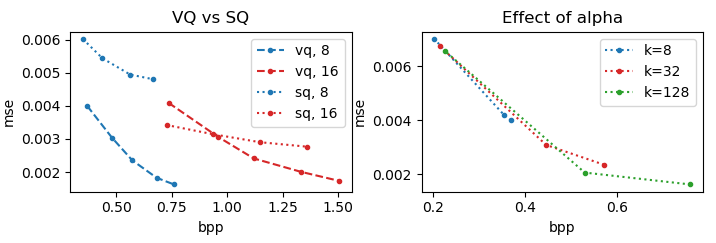
\includegraphics[scale=0.7]{figure1.png}
\end{center}
\caption{Rate-distortion curves. Rate is expressed in bits per pixel (bpp) of the original images, distortion is expressed in the mean squared error (mse) between the original and reconstructed images. See text for description.}\label{fig:plots}
\end{figure}

We next confirm the effectiveness of the soft cross-entropy term $s(\vc)$ in our final loss formulation in \eqref{eq:loss_final}.
Increasing the $\alpha$ hyper-parameter should put more importance on the rate minimization (through the entropy) as compared to the distortion.
In the right plot of figure \ref{fig:plots} we compare the points $k=[8, 32, 128]$ of the \emph{`vq, 8'} curve for values $\alpha = [0.01, 0.001, 0]$ from left to right.
With the highest $\alpha = 0.01$, the objective trade-off searches for the lowest rate tolerating higher distortion. The lower the $\alpha$, the less we push for low rates which allows for smaller distortion. 
This behaviour corresponds well to the expected and desirable one where, as formulated in \eqref{eq:trade_off}, we can now directly control the trade-off between between the two competing objectives by setting the hyper-parameter $\alpha$.

Examples comparing the original with the reconstructed images for the \emph{`vq, 8'} are available in the repo in the \href{https://bitbucket.org/dmmlgeneva/softvqae/src/master/paper/pics}{paper/pics} folder.
In the same place, there are examples of the learned $\qc$ histograms for \emph{`vq, 8, k=32'} with different values of $\alpha$.


% \subsubsection*{Acknowledgments}
% Use unnumbered third level headings for the acknowledgments. All
% acknowledgments, including those to funding agencies, go at the end of the paper.


\bibliography{softvqae}
\bibliographystyle{iclr2021_conference}

% \appendix
% \section{Appendix}
% You may include other additional sections here.

\end{document}
